%!TeX root = thesis-main.tex
 \emph{\scafi{} (Scala-Fields)} is
 an aggregate programming toolkit
 that comprises an internal DSL (language and virtual machine)
 as well as supporting components for the simulation
 and execution %deployment 
 of aggregate systems.

\subparagraph{Software description}
\label{}
\scafi{} is a multi-module Scala project hosted on GitHub\footnote{\url{https://github.com/scafi/scafi}}.
%
It provides DSL and API modules for 
 writing, testing, and running aggregate programs, namely programs expressed according to the aggregate programming paradigm~\cite{aggregatecomputing,DBLP:journals/jlap/ViroliBDACP19}.
%
\subparagraph{Software Architecture}
\label{sec:scafi-arch-design}

The high-level architecture of \scafi{} is depicted in \Cref{fig:scafi-arch}.
It consists of the following main components: %(where each component is an SBT module and deployable artifact):
\begin{itemize}
\item \texttt{scafi-commons} | provides basic abstractions and utilities (e.g., spatial and temporal abstractions);
\item \texttt{scafi-core} | provides an aggregate programming DSL (syntax, semantics, and a virtual machine for evaluation of programs), together with a ``standard library'' of reusable functions;
\item \texttt{scafi-stdlib-ext} | provides extra library functionality that requires external dependencies and is hence kept separated from the minimalist \texttt{scafi-core};
\item \texttt{scafi-simulator}: provides basic support for simulating aggregate systems;
\item \texttt{scafi-simulator-gui} | provides a GUI for visualizing and interacting with simulations of aggregate systems;
\item \texttt{spala} (``spatial Scala''---i.e., a general aggregate computing platform\footnote{aggregate computing is rooted in spatial computing~\cite{DBLP:journals/corr/abs-1202-5509}.}) | provides an actor-based aggregate computing middleware
(independent of the \scafi{} DSL and potentially applicable to other aggregate programming languages as well)
based on the Akka toolkit~\cite{akka};
\item \texttt{scafi-distributed} | ScaFi integration-layer for \texttt{spala},
which can be leveraged to set up actor-based deployments of \scafi{}-programmed systems.
\end{itemize}
 
\begin{figure}
\centering
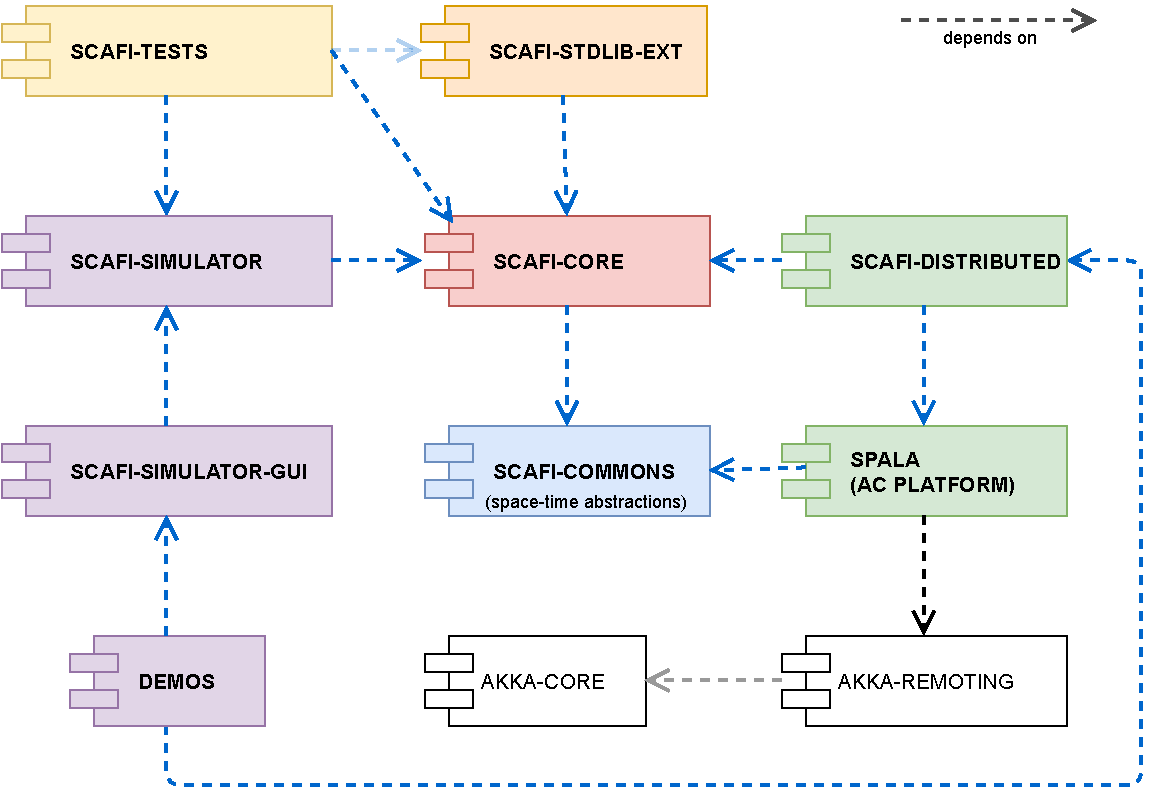
\includegraphics[width=0.8\textwidth]{papers/softwarex2021/imgs/scafi-project-org.pdf}
\caption{High-level architecture of the \scafi{} toolkit.}
\label{fig:scafi-arch}
\end{figure}

\begin{figure}
\centering
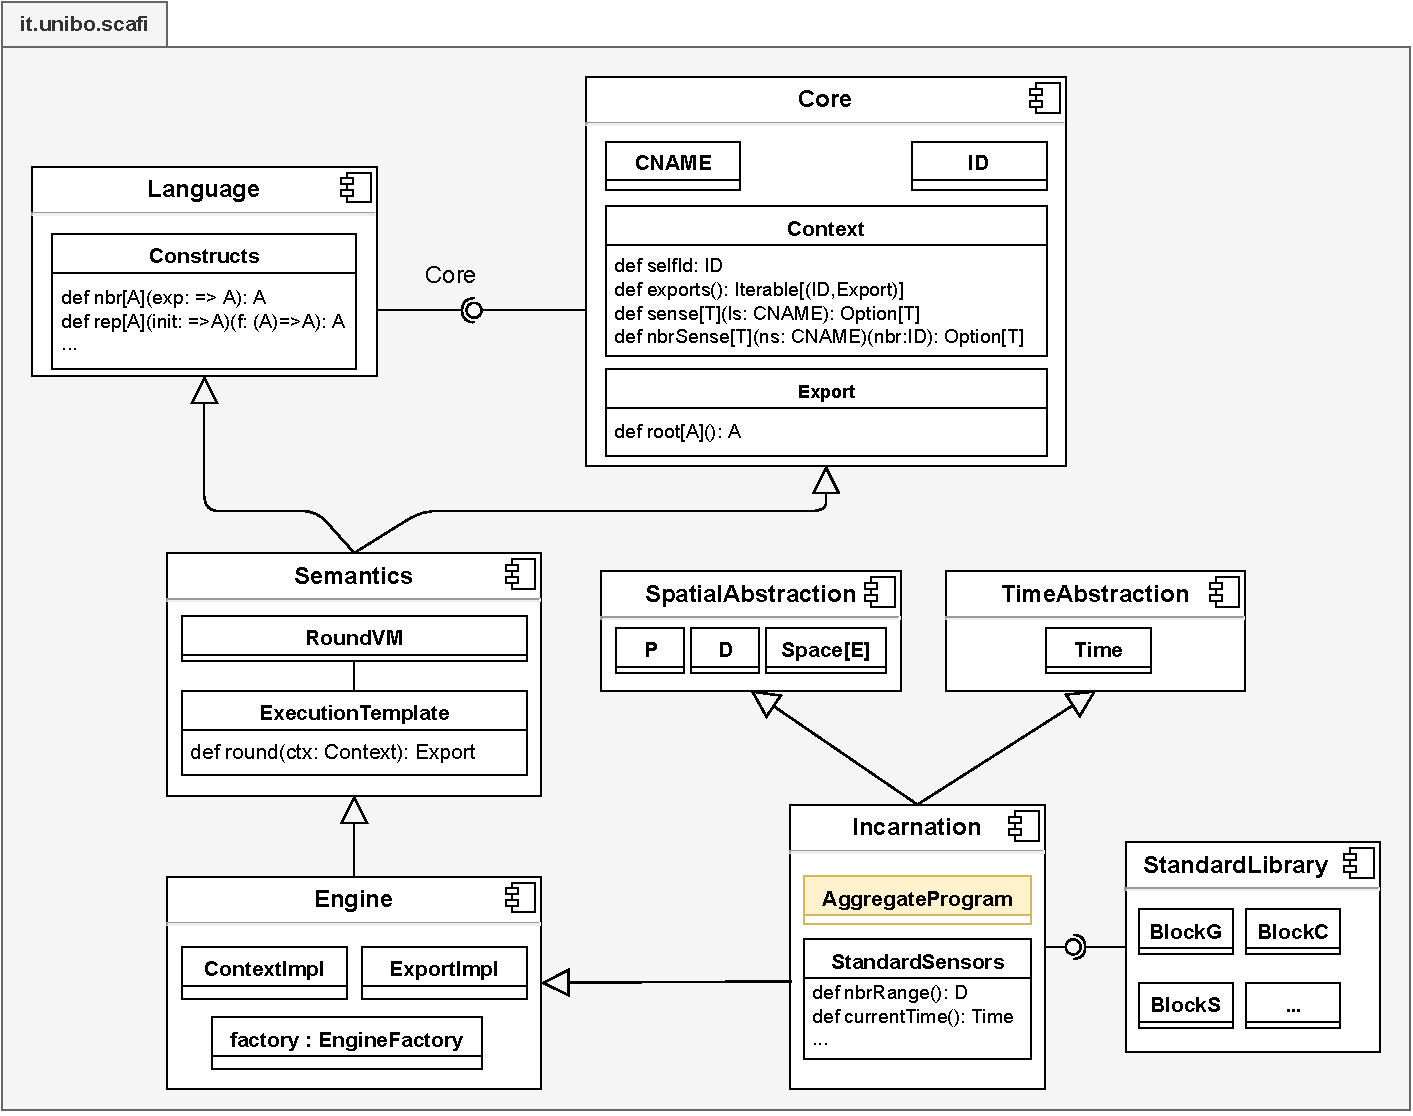
\includegraphics[width=0.8\textwidth]{papers/softwarex2021/imgs/scafi-design.drawio.pdf}
\caption{\revision{Design of the core of \scafi{} (DSL).}}
\label{fig:scafi-design}
\end{figure}

\revision{
\scafi{} leverages the concept of an \emph{incarnation},
 namely a concrete ``family of types''~\cite{DBLP:conf/oopsla/OderskyZ05} 
 that is progressively refined through inheritance, composed, and finally instantiated into an object (cf. the Scala \emph{cake pattern}~\cite{Hunt2013cakepattern,DBLP:conf/oopsla/OderskyZ05})
 which ultimately provides access 
 to a type-coherent set of features.

\Cref{fig:scafi-design} provides an excerpt 
 of the main Scala traits 
 with some types and objects they define.
%
Trait \texttt{Core} provides the abstract fundamental types: \texttt{CNAME} for capability names,
\texttt{ID} for device identifiers,
\texttt{Context} for the input environment of computation rounds,
and \texttt{Export} for the outcomes of computation rounds.
%
Trait \texttt{Language} 
 provides the syntax of the DSL in terms of methods, through interface \texttt{Constructs}.
%
Trait \texttt{Semantics} and \texttt{Engine}
 implement the DSL construct semantics,
 providing a template for \texttt{AggregateProgram} base class defined in the \texttt{Incarnation} trait. 
The incarnation also exposes \texttt{StandardSensors} in terms of, e.g., \texttt{SpatialAbstraction}'s and \texttt{TimeAbstraction}'s types for positions (\texttt{P}), distances (\texttt{P}), and time.
%
The \texttt{StandardLibrary} is provided by leveraging 
 what an incarnation provides,
 providing traits of functionality to be mixed into \texttt{AggregateProgram}s.
}

\subparagraph{Software Functionalities}
\label{}

\subparagraph*{Expressing aggregate programs through a Scala DSL}
\label{sec:express-programs}
%
Module \texttt{scafi-core}
 exposes,
 through incarnations,
 an \texttt{AggregateProgram} trait
  that provides access to 
  aggregate programming constructs---following 
  a variant of the field calculus~\cite{DBLP:journals/tocl/AudritoVDPB19,DBLP:journals/jlap/ViroliBDACP19}
  formalized in~\cite{DBLP:conf/isola/CasadeiVAD20}.
%
This single program defines -- from a global perspective -- 
 the collective adaptive behaviour 
 of an entire %system or 
 ensemble of computational devices.
%
Besides the core constructs,
 this module also provides ``standard library'' traits
 providing access to reusable functions of aggregate functionality.
%
For instance, by mixing trait \texttt{Gradients}
 into an \texttt{AggregateProgram} subclass,
 a developer gets access to \emph{gradient functions}~\revision{\cite{DBLP:conf/sac/BealBVT08,DBLP:journals/tomacs/ViroliABDP18}}, used to 
 continuously compute (over space and time) the self-healing field of minimum distances of each node from a set of source nodes. %---possibly in mobile and faulty environments.
%
Several such traits are available
 to provide other key building blocks
 for self-organising applications~\revision{\cite{DBLP:conf/saso/WolfH07,DBLP:journals/tomacs/ViroliABDP18}} (e.g., \texttt{BlockG} \revision{for gradient-wise information propagation}, \texttt{BlockC} \revision{for gradient-wise information collection}, \texttt{BlockS} \revision{for sparse choice or leader election})
 or experimental language features
 (e.g., the \texttt{spawn} function for concurrent aggregate processes~\revision{\cite{DBLP:journals/eaai/CasadeiVAPD21,testa2022processes}}\revision{, for modelling independent and overlapping aggregate computations}).
%
\subparagraph*{Virtual machine for the local execution of aggregate programs}
%
An \texttt{AggregateProgram} instance 
 is a function
 mapping a \texttt{Context}
 (the set of inputs needed by an individual device
  to properly evaluate the program locally)
 to an \texttt{Export}
 (the tree of values that has to be shared 
  with neighbours to effectively coordinate and promote 
  the emergence of collective behaviours).
%
Using this API,
 a developer can 
 integrate ``aggregate functionality''
 into its system---what remains to be specified are the
 details of the aggregate execution model and the communication among devices,
 that may change in different applications.
%
Devices must continuously run the aggregate program,
but the scheduling of these computation rounds can be tuned
as the application needs~\cite{DBLP:journals/lmcs/PianiniCVMZ21}.
%
\texttt{Export}s must be shared with neighbouring devices to allow them
to properly set up their \texttt{Context}s,
but the network protocol to be used to do so can be selected
independently of the program.
 
\subparagraph*{Simulation support}
%
In order to simulate an ``aggregate system'',
 it is necessary to: 
\begin{enumerate}
  \item define the set of computational devices that make up the aggregate, including their sensors and actuators;
  \item define the aggregate topology, i.e., 
  some application-specific \emph{neighbouring relationship}
  from which the set of \emph{neighbours}
  of each device can be determined;
  \item define the aggregate program to be executed;
  \item define a certain dynamics of the system
  by proper scheduling of computation rounds,
  and the environment
  by proper scheduling of changes in sensor values.
\end{enumerate}

%
Module \texttt{scafi-simulator}
 provides this basic support.
%
It exposes some factory methods
to configure simulations properly
 (e.g., it supports ad-hoc and spatial distance-based connectivity rules)
 and an API to run and interact with simulations.
%
Then, module \texttt{scafi-simulator-gui}
 provides a convenient graphical user interface
 to launch and visually show simulations in execution.
%
We remark that these modules currently support basic simulation scenarios
 and are mainly meant for quick experiments
 or as a starting basis for ad-hoc simulation frameworks.
 
\subparagraph*{Experimental or work-in-progress features: actor-based middleware}
%
Regarding the construction of actual systems, 
 \scafi{}
 provides
 an actor-based implementation
 of the aggregate execution model~\cite{DBLP:series/lncs/CasadeiV18},
 in the \texttt{spala} (\texttt{Spa}tial Sca\texttt{la}) module,
 which is instrumental for integrating aggregate computing
 into existing systems and distributed architectures~\cite{DBLP:series/lncs/CasadeiV18}.
%
Indeed, aggregate computing systems
 can be designed, deployed, and executed 
 according to different
 architectural styles 
 and concrete architectures~\cite{DBLP:journals/fi/CasadeiPPVW20}.
%
So, \scafi{} provides \emph{two} main implementations of the middleware,
 in package \texttt{it.unibo.scafi.distrib.actor},
 for purely peer-to-peer 
 (sub-package \texttt{p2p})
 and server-based designs
 (sub-package \texttt{server}).
%
The main abstraction
 is the \texttt{DeviceActor},
 which exposes a message-based interface
 for controlling and interacting with
 an individual logical node of the aggregate system.
%
Then, an object-oriented façade API is provided to set up a system of middleware-level actors. 

%\subparagraph{Sample code snippets analysis (optional)}
%\label{}

%\subparagraph{Illustrative Examples}
\label{sec:examples}
\subparagraph{Hello \scafi{}: building an aggregate system that computes a gradient, from scratch}
This complete example, shown in \Cref{fig:example-full} and available online\footnote{\url{https://github.com/scafi/hello-scafi}}, illustrates how it \scafi{} can be used
 to program a (simulated) aggregate system
 for computing a self-stabilising \emph{gradient} field~\cite{DBLP:conf/sac/BealBVT08,DBLP:journals/tomacs/ViroliABDP18}
 where the output of each device self-stabilises to
 its minimum distance from an appointed \emph{source} device.
%
Development comes in two parts:
\begin{enumerate}
  \item definition of the aggregate program,
  namely the logic of collective behaviour (\Cref{fig:example-full1})\footnote{For a detailed explanation of this gradient implementation, please refer to e.g. \cite{DBLP:journals/eaai/CasadeiVAPD21}.}~\footnote{Concerning source code listings, we highlight symbols as follows: we use blue for Scala keywords, red for \scafi{} DSL constructs, purple for \scafi{} library functions, and brown for other \scafi{} API symbols (e.g., types, objects, constants, and methods).};
  \item definition of an ``aggregate execution protocol''
  determining how devices communicate and act upon their environment (\Cref{fig:example-full2}).
\end{enumerate}

\begin{figure}
\newsavebox{\exoprogram}
\begin{lrbox}{\exoprogram}% Store first listing
\begin{lstlisting}[basicstyle=\lst@ifdisplaystyle\footnotesize\fi\ttfamily]
// 1. Define/import an incarnation, it provides ScaFi types and classes
object MyIncarnation extends
  it.unibo.scafi.incarnations.BasicAbstractIncarnation
// 2. Bring into scope the stuff from the chosen incarnation
import MyIncarnation._
// 3. Define an "aggregate program" using the ScaFi DSL 
// by extending AggregateProgram and specifying a "main" expression
class GradientProgram extends AggregateProgram {
  def isSource: Boolean = sense("source")
  override def main(): Any = rep(Double.PositiveInfinity)(d => {
    mux(isSource){ 0.0 } {
      foldhoodPlus(Double.PositiveInfinity)(Math.min){ nbr(d) + 1.0 } 
}})}
\end{lstlisting}
\end{lrbox}
\newsavebox{\exosystem}
\begin{lrbox}{\exosystem}% Store first listing
\begin{lstlisting}[deletekeywords={[2]{nbr}},
emph={state}, basicstyle=\lst@ifdisplaystyle\footnotesize\fi\ttfamily]
// 4. In your program, implement an "execution loop" whereby
// your device or system executes the aggregate program
object HelloScafi extends App {
  case class DeviceState(self: ID, exports: Map[ID, EXPORT],
      localSensors: Map[CNAME, Any], 
      nbrSensors: Map[CNAME, Map[ID, Any]]) {
    def updateExport(dev: ID, export: EXPORT): DeviceState = 
        this.copy(exports = exports + (dev -> export))
  }
  val devices = 1 to 5  // (1,2,3,4,5), i.e., 5 devices
  val sourceId = 2      // device 2 is the source of the gradient
  val scheduling = devices ++ devices ++ devices ++ devices ++ devices
  val program = new GradientProgram()
  def neighboursFrom(id: ID): Seq[Int] = // topology [1]-[2]-[3]-[4]-[5]
    Seq(id - 1, id, id + 1).filter(n => n > 0 && n < 6)
// Now let's build a simplified system to illustrate the execution model
  var state: Map[ID, DeviceState] = (for {
    d <- devices
  } yield d -> DeviceState(d, Map.empty, Map("source" -> false),
      Map(NBR_RANGE -> (neighboursFrom(d).toSet[ID]
        .map(nbr => nbr -> Math.abs(d - nbr).toDouble)).toMap))).toMap
  state = state + (sourceId -> state(sourceId).copy(localSensors =
      state(sourceId).localSensors + ("source" -> true))) // set source
// The cycle simulates scheduling&communication by read/write on `state`
  for(d <- scheduling){ // run 5 rounds for each device `d`, round-robin
    // build the local context for device d
    val ctx = factory.context(selfId = d, exports = state(d).exports,
      lsens = state(d).localSensors,nbsens = state(d).nbrSensors)
    println(s"RUN: DEVICE ${d}\n\tCONTEXT: ${state(d)}")
    // run the program against the local context
    val export = program.round(ctx)
    // update d's state
    state += d -> state(d).updateExport(d, export)
    // Simulate sending of messages to neighbours
    state(d).nbrSensors(NBR_RANGE).keySet.foreach(
      nbr => state += nbr -> state(nbr).updateExport(d, export))
    println(s"\tEXPORT: ${export}\n\tOUTPUT: ${export.root()}\n---")
  }
}
\end{lstlisting}
%  // Import standard sensors name defined in incarnation
%  val sensorsNames = new StandardSensorNames {}; import sensorsNames._
\end{lrbox}
\subfloat[\label{fig:example-full1}Program definition]{
\usebox{\exoprogram}
}\\
\subfloat[\label{fig:example-full2}System and execution definition]{
\usebox{\exosystem}
}
\caption{Complete example: an aggregate system computing a gradient.}
\label{fig:example-full}
\end{figure}
\subparagraph{Features}
\label{s:impact}
\scafi{}
 has been used 
 in aggregate computing-related research~\cite{DBLP:journals/eaai/CasadeiVAPD21,audrito2022ecoop-xc,DBLP:conf/coordination/AguzziCV22,
 DBLP:conf/fmec/CasadeiV19,DBLP:conf/IEEEscc/CasadeiTVD19,DBLP:journals/scp/CasadeiAV18,DBLP:journals/jsan/CasadeiAV21,DBLP:conf/coordination/CasadeiVRA21,casadei2022applsci,arxiv2020scafi-nc},
  touching themes such as 
  software engineering, 
  computational models, and
  distributed systems/algorithms.
%
The impact of \scafi{}
 can be understood in terms of 
 existing and prospective contributions, 
 discussed in the following.

\subparagraph*{Interplay between programming language design and foundational research} 
%
The implementation of the \scafi{} DSL
 has inspired a variant of the field calculus
 which arguably supports easier embeddability
 into mainstream programming languages~\cite{DBLP:conf/isola/CasadeiVAD20,arxiv2020scafi-nc}.

\subparagraph*{High-level programming models}
%
The previous discussion  
 makes the case for ``DSL stacking''~\cite{DBLP:conf/icsoft/HummE10}.
%
Indeed, by leveraging the aforementioned aggregate process extension, 
 it is possible to reduce the abstraction gap
 needed to implement \emph{situated tuples}~\cite{DBLP:conf/coordination/CasadeiVRA21}\revision{,
 which is a Linda-like model~\cite{DBLP:journals/toplas/Gelernter85} for coordinating processes where tuples and tuple operations are situated in space}.
%
By mapping high-level specifications into aggregate programs, it is sometimes straightforward to develop resilient distributed implementations---as in~\cite{DBLP:journals/jss/AudritoCDSV21},
 where translation rules from 
 spatial logic formulas
 to field calculus expressions
 enable seamless construction of decentralized monitors for such formulas.

\subparagraph*{Web-friendliness}
%
By leveraging Scala.js~\cite{DBLP:conf/scala/Doeraene18}, \scafi{} can be easily 
 accessed through JavaScript,
 which promotes cross-platform language design 
 and reuse of functionality in the browser
 (to support web applications without the need of server-side components).
%
This paved the path 
 to \scafiweb{}~\cite{DBLP:conf/coordination/AguzziCMPV21},
 a web playground for aggregate programming.
%